\section{Problem analysis}
\subsection{Internet of Things}
\subsection{Cloud based IoT platform}
What is a Cloud based IoT platform? 

\subsubsection{Google Cloud Platform}
\paragraph{Overview} 
\textit{Cloud Platform brings scale of infrastructure, networking, and a range of storage and analytics products you can use to make the most of device generated data.}\cite{website:gcp}
This is Google's own description of their IoT Cloud solution, and the references article is used for analysis in this section. \\

The platform can be divided into three basic components, the device, gateway, and cloud, each of which are characterized by the following: A \textit{device} is defined as hardware and software that directly interacts with the world, and are connected to a network and the Internet. A \textit{gateway} lets devices \textit{not} directly connected to the Internet reach a cloud service. The \textit{Cloud} is the \textit{endpoint} of device data, where it can be processed.\\

Several terms are used to describe what devices constitute, but the most important seems to be metadata and state information. Device metadata contains information such as ID and the date manufactured. The state information is basically the device status, such as "on"/"off". Furthermore devices must be associated with some security credentials for authentication. \textit{Telemetry} is the term for device data gathering, and is described as the \textit{eyes-and-ears data} the device collects in its environment. Once a device has been defined, telemetry can be sent to the Cloud Platform. As mentioned, a gateway can provide connection to the cloud, when e.g. protocol translation is needed. The Cloud Platform is the infrastructure for data management, which is depicted in figure \ref{fig:gcp:infrastructure}.

\begin{figure}[h!]
	\centering
	\includegraphics[width=0.7\textwidth]{figures/gcp/infrastructure.png}
	\caption{Diagram of the Google Cloud Platform IoT infrastructure}
	\label{fig:gcp:infrastructure}
\end{figure}

Google calls each of these components \textit{services}, and are categorized by their functionality and role in the infrastructure. Communication between the services are called \textit{pipelines}, which includes transforming, computing, combining, and moving data. The Cloud Platform also provides means for storing data in Google Firebase\cite{website:firebase}
and is especially used for continuously mirroring device states and exposing them to clients (See figure \ref{fig:gcp:firebase}).

\begin{figure}[h!]
	\centering
	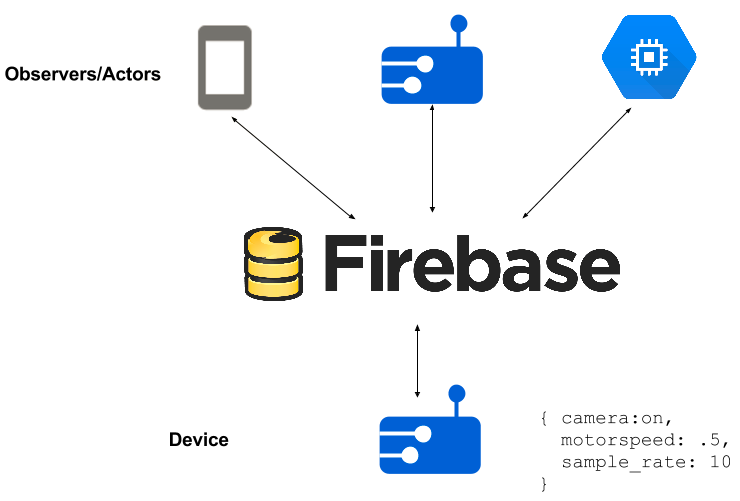
\includegraphics[width=0.5\textwidth]{figures/gcp/firebase.png}
	\caption{Abstract functionality of Google Firebase in the IoT Cloud Platform}
	\label{fig:gcp:firebase}
\end{figure}

The most interesting services are the "rule processing" and "streaming analytics", which allows for programmers to write custom logic for handling data triggered by device events. What you can do is to essentially trigger alerts, filter data, and invoke other APIs. This property of quick data processing is described as \textit{key} in the Cloud Platform. The "Cloud Dataflow" service provides means for \textit{more sophisticated} analytics. 

\paragraph{Services}
Google Cloud Platform is not just for IoT, but provides a plethora of products. The following is a list of the categories and \textit{some} of the services:

\begin{itemize}
	\item Compute: Compute Engine, App Engine, Cloud Functions
	\item Storage \& Databases: Cloud Storage, Cloud SQL
	\item Networking: Cloud Virtual Network
	\item Big Data: Cloud Pub/Sub, BigQuery
	\item Machine Learning: Cloud Machine Learning Platform, Cloud Natural Language API
	\item Identity \& Security: Cloud IAM, Cloud Resource Manager
	\item Management Tools: Monitoring, Logging, Trace, Cloud APIs
	\item Developer Tools: Cloud SDK, Cloud Deployment Manager
\end{itemize}

Some of the above mentioned services are self-explanatory, and some are just listed for reference. The IoT solution is a combination of only some of these services, and form the infrastructure explained in the overview. 

\subsubsection{Amazon Web Services}
\paragraph{Overview} \textit{AWS IoT is a managed cloud platform that lets connected devices easily and securely interact with cloud applications and other devices.}\cite{website:aws}.
Aside from the huge and popular web shop Amazon hosts, they have developed a huge library of web services, called "Amazon Web Services" (AWS). Above citation is from their website and describes one of their products; The "AWS IoT Platform". \\

AWS IoT Platform constitutes of several components, labeled "AWS IoT Device SDK", "Device Gateway", "Authentication and Authorization", "Registry", "Device Shadows", and "Rules Engine". The infrastructure is depicted in figure \ref{fig:aws:infrastructure}. \\

\begin{figure}[h!]
	\centering
	\includegraphics[width=\textwidth]{figures/aws/infrastructure.png}
	\caption{Components of AWS IoT Platform and the infrastructure}
	\label{fig:aws:infrastructure}
\end{figure}

The \textit{AWS IoT Device SDK} provides software development kits to connect hardware devices or mobile applications, and supports C, JavaScript, and Arduino. Protocols like MQTT, HTTP, and WebSockets are supported for connectivity and data exchange. Furthermore Amazon has partnered up to offer a wider variety of SDKs, including Google's Android and Apple's iOS. The SDKs are meant for making integration with AWS easier for the programmer by encapsulating operations on the IoT Platform in library function calls. 

The \textit{Device Gateway} provides before mentioned protocols for communication between devices and the IoT Platform. It can be configured to work as a publication/subscription model for one-to-one and one-to-many communication, and it even scales automatically with \textit{over a billion} devices connected.

Security is taken seriously by Amazon, and this is what \textit{Authentication and Authorization} takes care of. Data between device and IoT Platform is never exchanged without proven identity, by use of "SigV4" and X.509 certificates. It's possible to fully manage mapping of authentication policies for connected devices, as well as revoking access rights at any time. Another feature is to use Amazon Cognito, which basically takes care of authentication for mobile applications.

The \textit{Registry} tracks device metadata by establishing unique identities for connected devices. 

\textit{Device Shadows} are persistent, virtual versions of connected devices and represent their sates. This allows for other devices to interact with other devices through a REST API. In other words, it is a convenient way of updates devices, as well as getting information about them. 

The data processing happens in the \textit{Rules Engine}, which evaluates messages passed to IoT Platform by user defined rules. The data can simply be transformed and passed to another device, or routed to other AWS cloud services for further processing. This includes several of the AWS services like AWS Lambda, S3, and DynamoDB. \\

Figure \ref{fig:aws:example} is an example of the IoT Platform and illustrates how a light bulb can controlled through above mentioned services. A mobile application sends instructions to a controller, which communicates with the IoT Platform in the cloud. Two rules are defined to act upon triggered events. One rule routes the data to other AWS services for evaluation, and the other changes the light color of the bulb. In either case the device shadow is updated with a new state. If the light bulb is turned off, requested device states are still saved in the device shadow.  
\begin{figure}[h!]
	\centering
	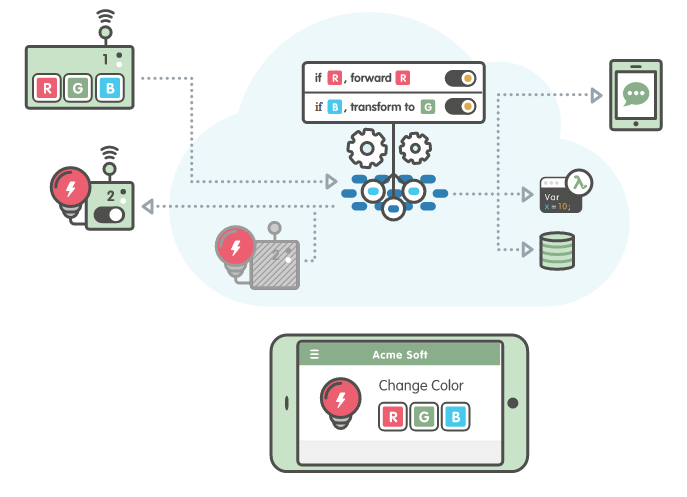
\includegraphics[width=\textwidth]{figures/aws/example.png}
	\caption{An AWS IoT Platform example illustrating the workings of the services.}
	\label{fig:aws:example}
\end{figure}

\paragraph{Services}
As mentioned in the overview, the Rules Engine allows for inbound data to be routed to other services. One worth mentioned is AWS Lambda, which executes computations in the cloud. It is even possible to write code in e.g. C\# and upload code snippets to the project. This service has the property of removing the need for a serer, as well as automatically scaling with the size of the workload. Other services like "DynamoDB" offers a NoSQL cloud database, and "Kinesis" for data analytics.  

\subsection{Microsoft Azure}
\textit{Azure IoT Hub is a fully managed service that helps enable reliable and secure bi-directional communications between millions of devices and a solution back end.} REF(https://docs.microsoft.com/en-us/azure/iot-hub/iot-hub-devguide)

Microsoft is another big player in the field of IoT Cloud computing, and offers their own IoT platform. Much confusingly they offer an IoT \textit{Suite}, as well as an IoT \textit{Hub}. The difference is that the IoT Suite is \textit{a collection of preconfigured solutions} REF(https://docs.microsoft.com/en-us/azure/iot-hub/iot-hub-what-is-azure-iot). This means that they have actually made customizable solutions based on common IoT scenarios, such as remote monitoring and asset management. The IoT Suite is however also the platform including the IoT Hub, which is the most important service in the IoT infrastructure, as it takes care of bidirectional connection with devices and the cloud. Figure REF(https://docs.microsoft.com/en-us/azure/iot-hub/iot-hub-what-is-iot-hub) illustrates the infrastructure of the platform from a device to the back end services. 

The IoT Hub keeps records of so called "Device twins", which are JSON documents containing device state and metadata information, for all connected devices. An identity registry enables devices to authenticate securely to the IoT Hub, which allows for full control of connecting devices. Devices communicate with the cloud though a device SDK or \textit{gateway}. The gateway is meant to be used when the offered SDKs do not support the device. Two types of gateways are offered, one being the \textit{protocol} gateway and the other being the \textit{field} gateway. The former is deployed in the cloud and performs protocol translation for MQTT, AMQP, and HTTP. The latter is deployed locally, i.e. physically close to the device(s), and enables also protocol translation, but also has the property of being able to actively manage devices, and the information mediated to the cloud. \\


\paragraph{Services}
Returning to the IoT Suite, a handful of services like Azure Stream Analytics, Storage, DocumentDB, WEb Apps, and Power BI are available for integration with the IoT Hub. Together they provide means for data analytics, storage, visualization, and integration with back-office systems. REF(https://docs.microsoft.com/da-dk/azure/iot-suite/iot-suite-overview). Telemetry can be routed to an Azure service by user-defined rules in the IoT Hub, and requires no code. As mentioned the IoT Suite contains preconfigured solutions, which are labeled "Remote monitoring" and "Predictive maintenance". These solutions are the way to start building an IoT platform, and are customizable and extensible. 

\subsection{IBM Watson IoT}
\textit{Watson IoT Platform is designed to simplify cognitive IoT development so you can harness the full potential of the Internet of Things} REF(https://www.ibm.com/internet-of-things/).

IBM has a lot of different domain specific products and solutions in regards to IoT. They offer different solutions based on the business application, e.g. "Asset management", "Facilities management", and "Product development" REF(https://www.ibm.com/internet-of-things/iot-solutions/). They are all hosted on the IBM Bluemix cloud platform, which essentially is a big collection of offered products and services for cloud computing. One of them is the Watson IoT Platform, which provides a "powerful application access to IoT devices and data to help you rapidly create analytics applications, visualization dashboards, and mobile IoT apps" REF(https://console.ng.bluemix.net/docs/starters/IoT/iot500.html).  

Watson IoT Platform offers two ways for data analytics; "Boards and cards" and "Rules and actions".

% Lightweight platforms:
%- PubNub

\subsection{Alternatives}